\documentclass{article}
\usepackage[table]{xcolor}
\usepackage{float}
\usepackage{array}
\usepackage{graphicx}
\usepackage[spanish, es-tabla]{babel}
\usepackage[utf8]{inputenc}
\usepackage{csquotes}
\usepackage[margin=1.55cm]{geometry}
\usepackage{wallpaper}
\usepackage[depth=3]{bookmark}
\usepackage[
backend=biber,
style=numeric,
]{biblatex}
\addbibresource{references.bib} 
\setlength{\parskip}{1em}
\parindent 0px

\newcolumntype{P}[1]{>{\centering\arraybackslash}p{#1}}
\newcolumntype{M}[1]{>{\centering\arraybackslash}m{#1}}
 

\newcommand\signature{
\noindent\begin{minipage}{10cm}
    \noindent\vspace{3pt}\par
    Firma: \rule{7cm}{1pt}
    \noindent\vspace{15pt}\par
\end{minipage}}

\begin{document}

\begin{titlepage}


    \ThisLRCornerWallPaper{1}{imgs/fondo_tt.png} % Fondo de portada 
        \begin{center}
            \LARGE \textbf{Instituto Politécnico Nacional}\\*[0.3cm]
            \Large \textbf{Escuela Superior de Cómputo}\\
            \vspace{1cm}
            \rule{12cm}{0.5mm}\\*[0.3cm]% Línea {Longitud}{Grosor}
            \hspace{0.9cm} 
            %\normalsize {\textit{Ingeniería en Sistemas Computacionales}}\\
            %%%%  TITULO Y NÚMERO DE TRABAJO   %%%%
    		\LARGE \textbf{ Aplicación móvil gamificada de aritmética\\}
    		\LARGE \textbf {\emph{Trabajo Terminal No }} 
    		\vspace{1cm} %Espacio vertical
    	\LARGE \textbf{\\ Ingeniería en Sistemas Computacionales\\}
    	Alumnos: *Pineda Vieyra Itzcoatl Rodrigo, Mothelet Delgado Izaird Alexander\\
	Directores: Elena Fabiola Ruiz Ledesma, Lorena Chavarría Baez\\
	e-mail: itzcoatlpv@gmail.com
    \vspace{1cm} %Espacio vertical
        \end{center}

    \centering %Todo centrado
    \vspace{1cm} %Espacio vertical

    %%%%   ALUMNOS   %%%%
   	


\end{titlepage}

\tableofcontents

\section{Introducción}

\subsection{Motivación}
\subsection{Plantamiento del Problema}
\subsection{Objetivos}
\subsubsection{Objetivo General}Desarrollar una aplicación móvil que apoye al estudiante de nivel medio superior en la 
adquisición de habilidades y conocimientos elementales, para fortalecer la destreza 
operatoria en  Aritmética, con el uso de la gamificación.

\subsubsection{Objetivos Específicos}
\begin{itemize}
	\item Diseñar actividades gamificadas, empleando números enteros y fraccionarios con las 4 operaciones básicas.
	\item Diseñar la arquitectura de la aplicación.
	\item Validar la aplicación móvil. 
\end{itemize}
\subsection{Estado del Arte}
\subsection{Propuesta de Solución}
\section{Marco Teórico}
\subsection{Motivación}
La motivación se refiere a los procesos que influencian la incitación, fuerza y dirección del comportamiento. “Estar motivado significa estar movido a hacer algo” \cite{ryan2000self}. Los psicólogos distinguen la motivación intrínseca (hacer algo por gusto o interés propio) y la extrínseca (actuar porque lleva a un resultado separable).
La motivación intrínseca ha sido estudiada exhaustivamente en las últimas décadas, particularmente sus aplicaciones en educación, resultando en evidencia de que la motivación intrínseca resulta en aprendizaje de alta calidad y creatividad \cite{albrecht2018relevance}.
En cuanto a la motivación extrínseca se suele tomar las ideas de la teoría del conductismo al condicionar un comportamiento a través de consecuencias. Se puede reforzar dicho comportamiento mediante premios, cuando una acción da un premio se repetirá esa acción \cite{escribano2010gamification}.
Una de las teorías más populares y estudiadas es La Teoría de la Autodeterminación (SDT, por sus siglas en inglés), la cual presenta un marco amplio  para el estudio de la motivación y la personalidad humanas. SDT articula una metateoría para enmarcar estudios motivacionales. Establece también una teoría formal que define fuentes intrínsecas y extrínsecas de motivación, sus roles y los  tipos de motivación extrínseca en el desarrollo cognitivo y social. Los autores Deci y Ryan consideran que comprender los distintos tipos de motivación extrínseca y lo que las promueve, es un asunto importante para educadores, quienes no siempre pueden contar con motivación intrínseca para fomentar el aprendizaje. Principalmente porque muchas de las tareas que los educadores esperan de los alumnos no son inherentemente interesantes o disfrutables, por lo que saber cómo promover formas más activas y volicionales, en lugar de pasivas y controladoras, se vuelve una estrategia esencial para la enseñanza [27]\\.
Dentro de SDT se encuentra la Teoría de la Integración Organísmica (OIT: Organismic integration Theory), la cual detalla las diferentes formas de motivación extrínseca y los factores contextuales que la promueven o dificultan.\\      
         
La figura 3 ilustra los diferentes tipos de motivación propuestos por OIT. Al extremo izquierdo se tiene la desmotivación, la cual se define como “el estado de falta de intención de actuar”. El comportamiento de alguien desmotivado carece de intencionalidad y de un sentido de causalidad personal. La desmotivación es el resultado de no valorar una actividad, no sentirse competente para realizarla, o no creer que producirá el resultado deseado.\\

\begin{figure}[h]
    \centering
    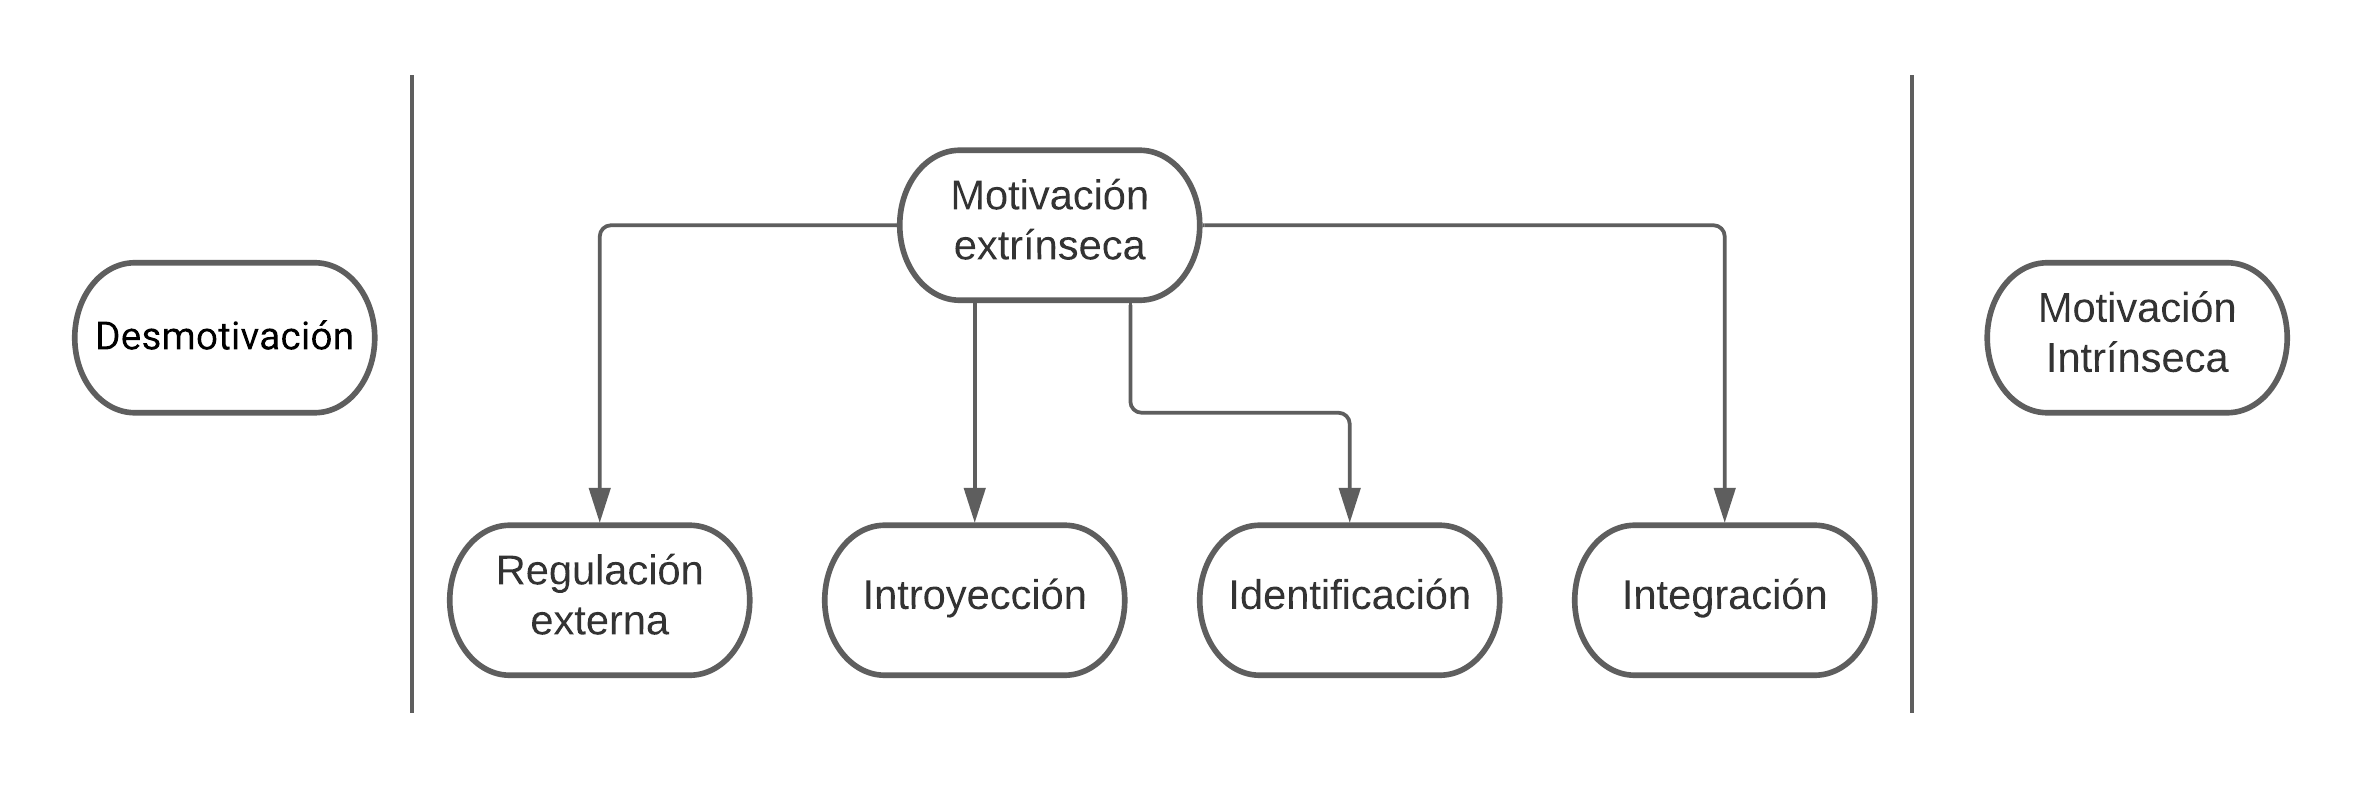
\includegraphics[scale=1]{imgs/MotivacionDiagrama.png}
    \caption{Tipos de motivación}
\end{figure}
A la derecha de desmotivación se encuentra la categoría menos autónoma de motivación extrínseca denominada regulación externa. Estos comportamientos son realizados para satisfacer una demanda externa u obtener una recompensa.
El segundo tipo de motivación extrínseca es la regulación introyectada. La introyección se refiere a un tipo de regulación interna que sigue siendo muy controladora porque la gente hace esas acciones con sentimientos de presión para evitar culpa o ansiedad o para lograr aumentar el ego u orgullo. 
Una forma más autodeterminada de motivación extrínseca es regulación a través de identificación. La identificación ocurre cuando la persona ha identificado la importancia personal de un comportamiento y, por tanto, ha aceptado su regulación como propia.
Finalmente, la forma más autónoma de motivación extrínseca es la regulación integrada.La integración ocurre a través de auto examinación y la asimilación de nuevas regulaciones con el resto de los valores y necesidades del individuo. Entre más se internalicen las razones para una acción y las asimile uno mismo, más se vuelven autodeterminadas las acciones motivadas extrínsecamente \cite{ryan2020intrinsic}.
Es importante recalcar que esta escala no significa que la motivación empiece en desmotivación y progresivamente avance, se puede empezar en cualquier nivel y mover según distintos factores.
Esta teoría es relevante para el proyecto en proceso y que se reporta en el presente documento,  porque explora los orígenes de la motivación. Si bien se planea atraer a los usuarios con recompensas, el objetivo es que conforme usen la aplicación los usuarios asimilen la utilidad del desarrollo de la destreza operatoria. 


\subsection{Gamificación}
\section{Análisis}
\subsection{Requisitos Funcionales}
\begin{enumerate}
%\item{Funcionalidad que se desarrolló}
\item {El sistema permitirá el registro se realizará por medio de un correo y contraseña válidos}
\item{El sistema permitirá el ingreso de un usuario al sistema mediante un correo y contraseña válidos previamente registrados}
\item {}
\end{enumerate}
\subsection{Requisitos No Funcionales}
\subsection{Casos de Uso}
\subsubsection{Tabla descriptiva de Caso de Uso 1}
\begin{tabular}{|M{5cm}|c|}
\hline
Caso de Uso & CU1 Registrar Usuario\\ \hline
Versión & 1.1\\ \hline
Autor(es) & Itzcoatl Rodrigo Pineda Vieyra\\ \hline
Revisor & Izaird Alexander Mothelet Delgado \\ \hline
Actor(es) & Usuario Final \\ \hline
Entradas & nickname, correo electrónico, contraseña, escolaridad\\ & Cuenta de Google \\ \hline
Salidas & Cuenta de usuario creada \\ \hline
Pre-condiciones & Instalar y abrir la aplicación \\ \hline
Post-condiciones & Cuenta de usuario creada\\ \hline
Mensajes & MSN1: "Ingrese un texto válido"\\
		 & MSN2: "Bienvenido"\\ \hline
Fuente & RF1 \\ \hline	
	Trayectoria & Trayectoria A (principal)\\
		& 1.   El usuario seleccionará la opción de registrarse.\\
		& 2.   Se ingresarán los datos correspondientes.\\
		& 3.   Se creará correctamente la cuenta del usuario\\
	& Trayectoria B\\
	& 1.   El usuario seleccionará la opción de registrarse.\\
	& 2.   Se proporcionará una cuenta de Google\\
	& 3.   Se confirma y se dan los permisos corresponddientes.\\
	& 4   Se creará correctamente la cuenta del usuario.\\ \hline
\end{tabular}
\subsubsection{Tabla descriptivad de Caso de Uso 2}
\begin{tabular}{|M{5cm}|c|}
\hline
Caso de Uso & CU2 Iniciciar Sesión\\ \hline
Versión & 1.1\\ \hline
Autor(es) & Itzcoatl Rodrigo Pineda Vieyra\\ \hline
Revisor & Izaird Alexander Mothelet Delgado \\ \hline
Actor(es) & Usuario Final \\ & Administrador\\ \hline
Entradas &  Correo electrónico, contraseña\\ & Cuenta de Google \\ \hline
Salidas & Sesión de usuario \\ \hline
Pre-condiciones & Instalar y abrir la aplicación \\ \hline
Post-condiciones & Sesión iniciada\\ \hline
Mensajes & MSN1: "Ingrese un texto válido"\\
		   & MSN2: "Bienvenido"\\ \hline
Fuente & RF1 \\ \hline	
	Trayectoria & Trayectoria A (principal)\\
		& 1.   El usuario ingresa sus credenciales (correo y contraseña).\\
		& 2.   Se valida si existen coincidencias de las credenciales proporcionadas\\
		& 3. Se inicia sesión o se despliega un mensaje de error.\\
	& Trayectoria B\\
	& 1.   El usuario seleccionará la opción de registrarse.\\
	& 2.   Se proporcionará una cuenta de Google\\
	& 3.   Se inicia sesión.\\ \hline
\end{tabular}

\subsection{Análisis de Interfaces}
%Descripcion de tipo de interfaz y por que
Las interfaces deberán ser optimizadas para dispositivos móviles. Deberá considerarse la capacidad touch de dichos dispositivos. La primera pantalla será para Iniciar sesión por medio del correo y contraseña junto con un botón para registrarse. La pantalla de registro solicitará el correo, contraseña y confirmación de la contraseña. Se deberá contar con botones para acceder al perfil de usuario, leaderboards y logros en una barra de navegación, esta puede ser horizontal o vertical. La pantalla de ejercicios mostrará la puntuación en todo momento en una esquina y el número de respuestas correctas consecutivas junto un icono. En caso de haber tiempo para responder a una pregunta habrá una barra horizontal en la parte superior la cual irá desapareciendo conforme transcura el tiempo asignado al usuario para dar respuesta a la pregunta, la cual irá  desaapareciendo de derecha a izquierda.
\subsection{Análisis de la Base de Datos}%Narrativa
Para desarrollar esta aplicación se cuenta con una entidad Usuario con campos correo (llave primaria) y contraseña, con el correo como identificador de la entidad, pues no se permiten correos duplicados.
\subsection{Tecnologías usadas}
\pagebreak
\section{Diseño}
\subsection{Arquitectura general del sistema}%Imagen arquitectura y descripcion%Imagen arquitectura y descripcion
La arquitectura se compone de 6 módulos (ver figura 2).  El primer módulo es el de Registro de Usuario y es el encargado de dar de alta y validar a los usuarios. El segundo módulo corresponde a la lista de ejercicios que el usuario puede realizar, los cuales se obtienen de la base de datos de ejercicios. El módulo evaluador de logros y mecánicas, que lleva el control de los logros y actividades gamificadas, lleva el control de la puntuación y los niveles de dificultad. Las estadísticas y progreso del usuario son registradas por el módulo correspondiente. El módulo generador de problemas es donde el administrador crea las plantillas de los ejercicios y actividades, los cuales son almacenados en su respectiva base de datos. Estas plantillas son usadas por dicho módulo para generar expresiones aritméticas las cuales son evaluadas por el módulo Evaluador de expresiones.  
\begin{figure}[H]
    \centering
    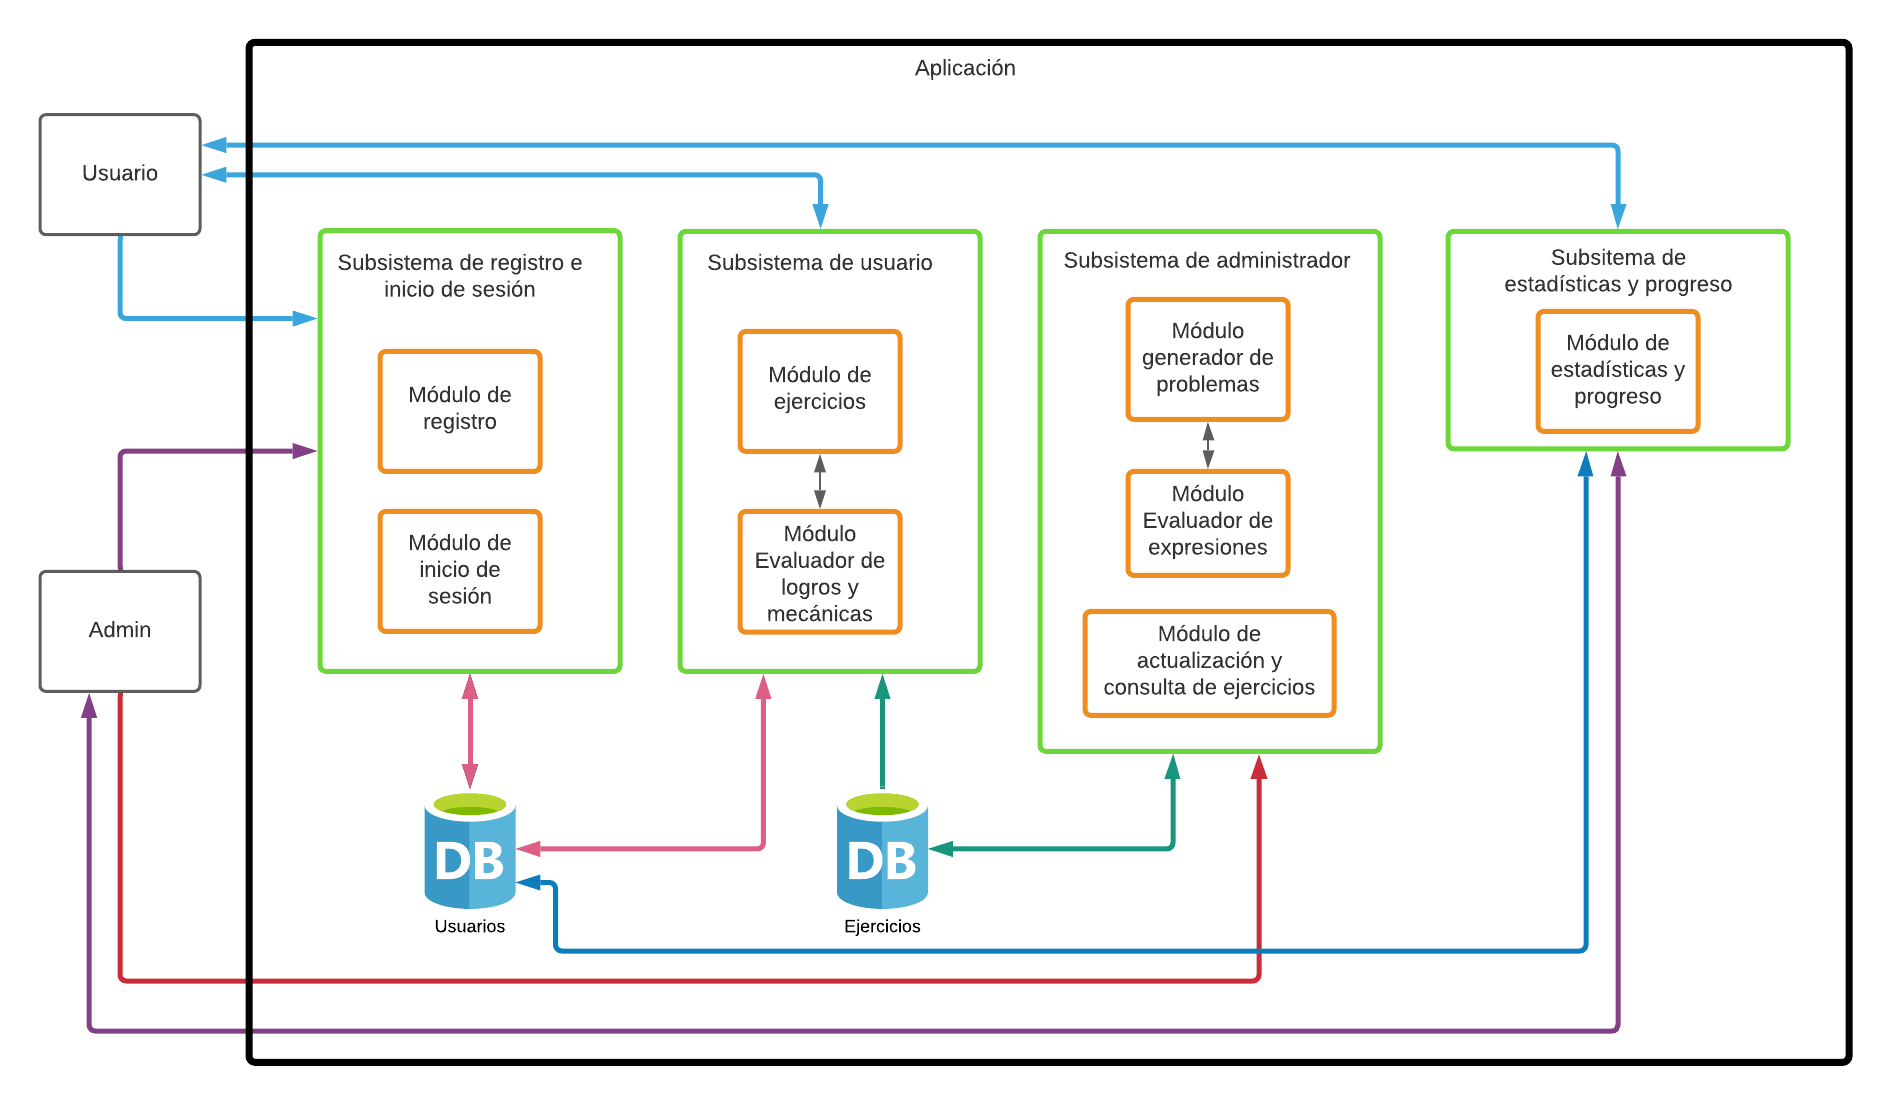
\includegraphics[scale=0.7]{imgs/Arquitectura}
    \caption{Arquitectura}
\end{figure}

\subsection{Diseño de Base de Datos}%diagrama entidad relacion pk subrayada
\begin{figure}[H]
    \centering
    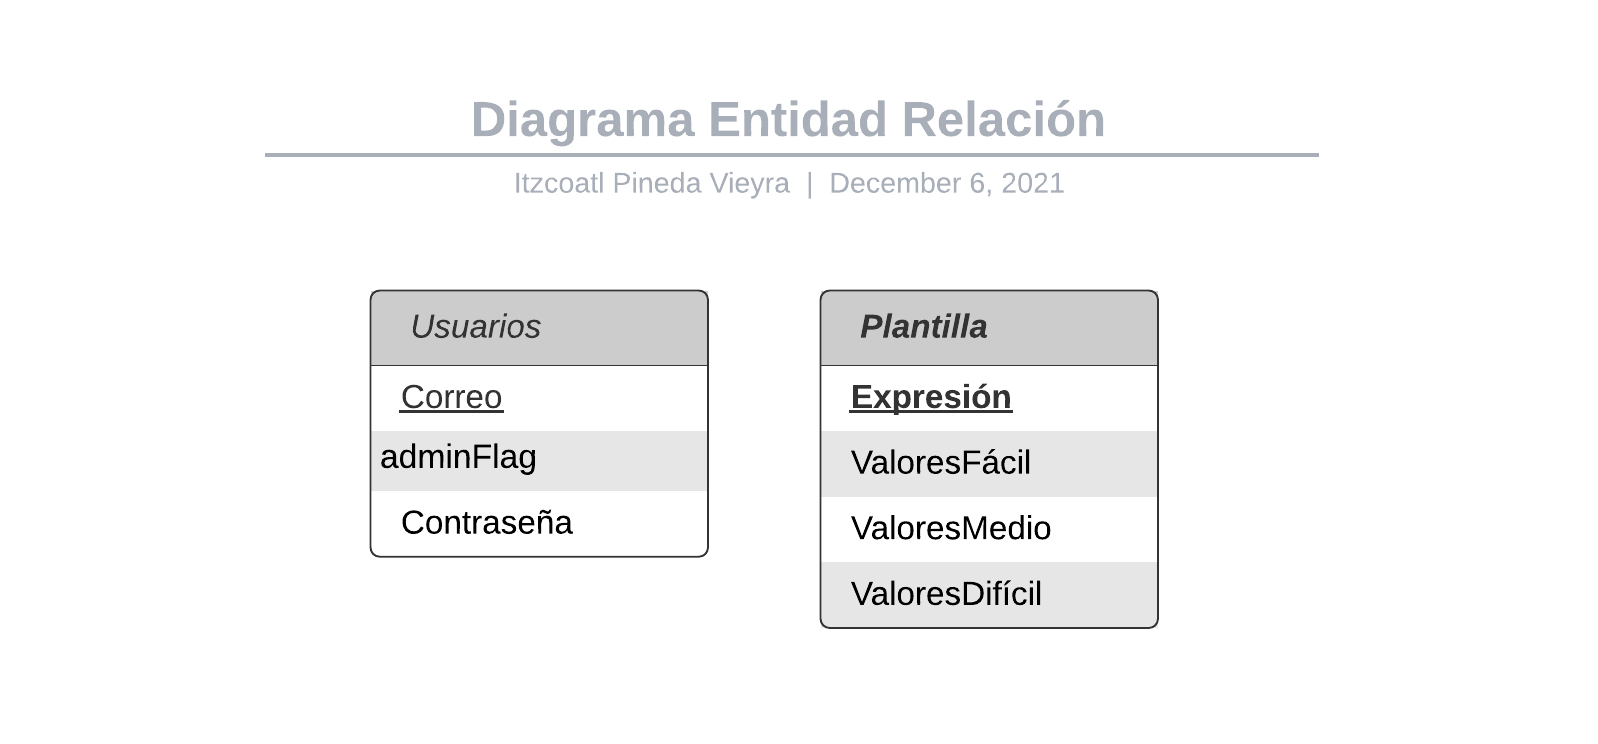
\includegraphics[scale=0.9]{imgs/BSD}
    \caption{Diagrama entidad relación}
\end{figure}
\subsection{Diseño de Interfaces}%mock-ups
En este apartado se presentarán los ddiseños de las interfaces previamente descritras.
\pagebreak
\begin{figure}[H]
    \centering
    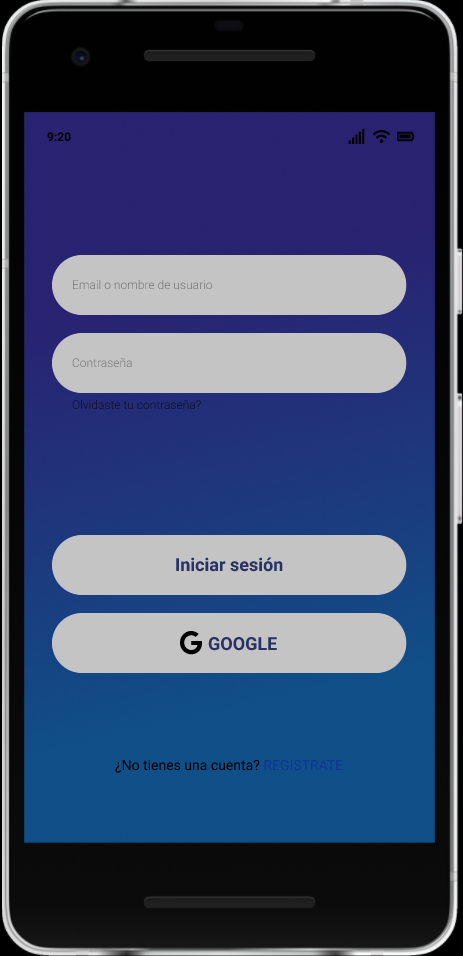
\includegraphics[scale=0.9]{imgs/Figma/Login}
    \caption{Login}
\end{figure}
\begin{figure}[H]
    \centering
    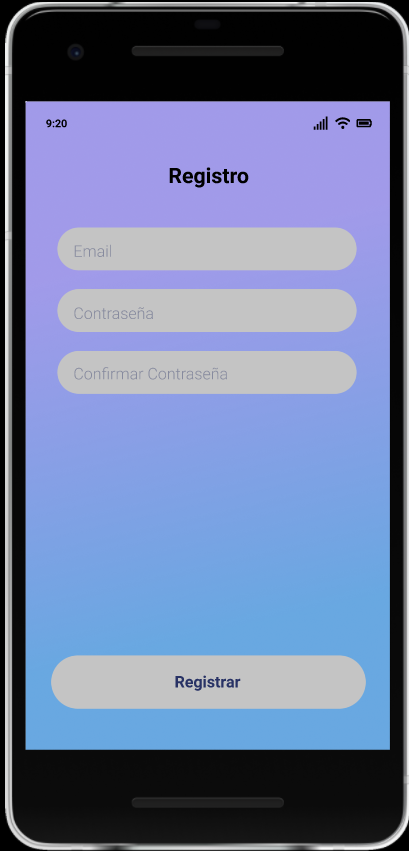
\includegraphics[scale=0.9]{imgs/Figma/Registro2}
    \caption{Registro}
\end{figure}
\subsection{Metodología}
\pagebreak
\section{Implementación}
%Subsistema de registro e ingreso Captura de pantalla con descripcion citar mock up de la pantalla
El subsistema de registro e ingreso fue implementado con Firebase 
\begin{figure}[H]
    \centering
    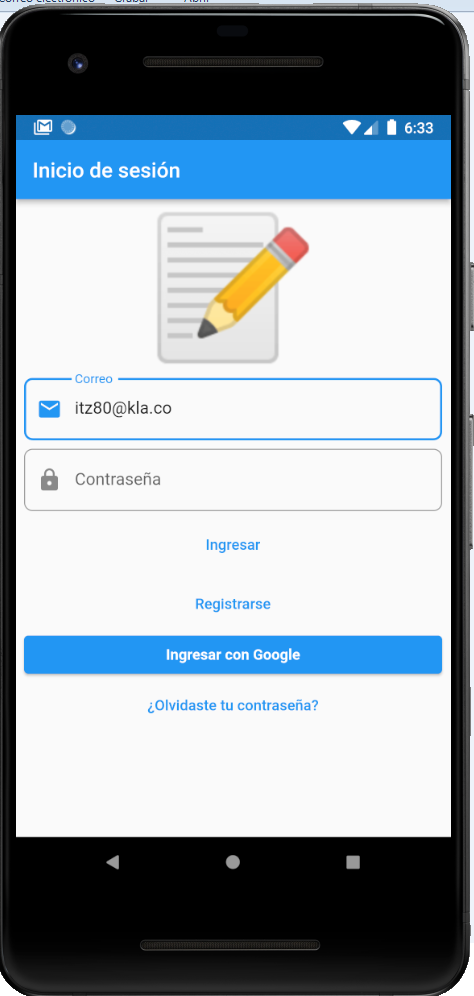
\includegraphics[scale=0.8]{imgs/Imp/Login1}
    \caption{Implementación de Login}
\end{figure}
\begin{figure}[H]
    \centering
    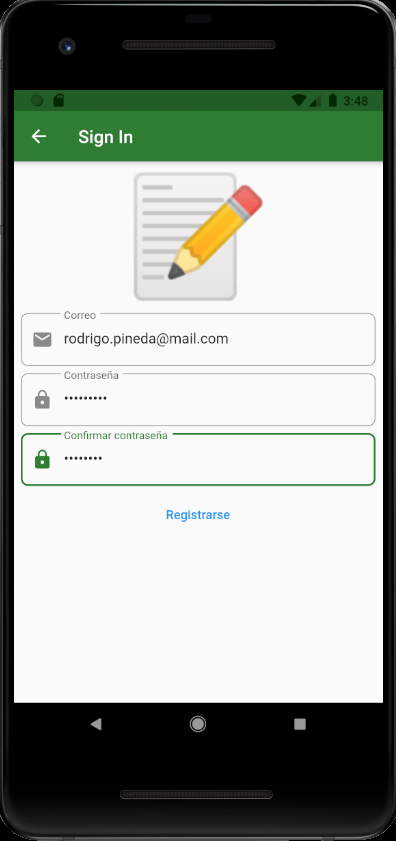
\includegraphics[scale=0.8]{imgs/Imp/Registro}
    \caption{Implementación Registro}
\end{figure}
\section{Pruebas}%Que pruebas se le hicieron al sistema
Se validó el correo con una expresión regular. Algunos ejemplos de correos validos
\begin{itemize}
	\item itz80@kla.co
	\item \verb |itz!&*%^7@protonmail.net|
	\item 1A!e@protonmail.com
\end{itemize}

\pagebreak
\printbibliography


\end{document}